\noindent\textbf{Matriz de confucion para los modelos}\\

En la tabla \ref{tab:mejores_prompts_modelos} se encuentra el mejor prompt segun su Aproximated Acuraccy de cada modelo. En esta tabla se puede observar que no hay un prompt que destaque en para todos los modelos, tampoco se puede encontrar una estrategia de prompting que sea ampliamente superadora a las demas, ya que esta tabla sugiere que varios modelos mejoran con 2-shot, pero no es definitiva para todos los modelo.

En el grafico \ref{fig:matriz_confucion} se encuentran las matrices de confucion para los experimentos anteriores, cada modelo con su mejor prompt. Se puede observar que cada modelo mantiene la tendencia que se ve en el grafico \ref{fig:bias}. Ademas se puede hacer foco en que es lo que no se desea en los modelos, lo primero es que su matriz de confucion sea disperza como la matriz de Llama 3.2 3B y lo segundo es que hay algunos errores que son peores que otros, por ejemplo clasificar un texto como A2 siendo que su clasificacion original es C2 es un error mas severo que clasificar textos como B1 siendo originalmente A2, tanto por la proximidad como por la relacion de dificulad (una persona con nivel B1 deberia poder interpretar correctamente un texto de A2).

\begin{table}[]
\centering
\begin{tabular}{@{}ccccc@{}}
\toprule
Orden & Modelo                  & Prompt    & Aproximated Acuraccy & Accuracy \\ \midrule
1     & B) Fine-tuning Adaptado & Prompt 2  & 0.936               & 0.872    \\
2     & B) Fine-tuning          & Prompt 2  & 0.923               & 0.846    \\
3     & C) DeepSeek             & Prompt 18 & 0.718               & 0.513    \\
4     & C) Chat GPT             & Prompt 17 & 0.679               & 0.436    \\
5     & D) Cathoven             & Prompt 25 & 0.654               & 0.436    \\
6     & A) Llama 3.1 8B         & Prompt 15 & 0.641               & 0.462    \\
7     & A) Llama 3.2 11B        & Prompt 16 & 0.628               & 0.436    \\
8     & D) Text Inspector       & Prompt 25 & 0.628               & 0.436    \\
9     & A) Mistral 12B          & Prompt 18 & 0.615               & 0.487    \\
10    & A) Gemma 2 9B           & Prompt 11 & 0.590               & 0.410    \\
11    & A) Llama 3.2 3B         & Prompt 10 & 0.577               & 0.462    \\
12    & A) Mistral 8B           & Prompt 1  & 0.538               & 0.333    \\ \bottomrule
\end{tabular}
\caption{Mejor prompt para cada modelo segun la Aproximated Acuraccy, para la particion de evaluacion}
\label{tab:mejores_prompts_modelos}
\end{table}

\todo{dejar propmt 25 o cambiarlo a que no acepta prompt, conviene poner el orden absoluto o relativo en la tabla?}
%el orden relativo es el que esta, el absoluto es el orden que ocupa cada experimento (modelo + prompt) de la lista completa de exprimentos.

\begin{figure*}[]
  \centering
  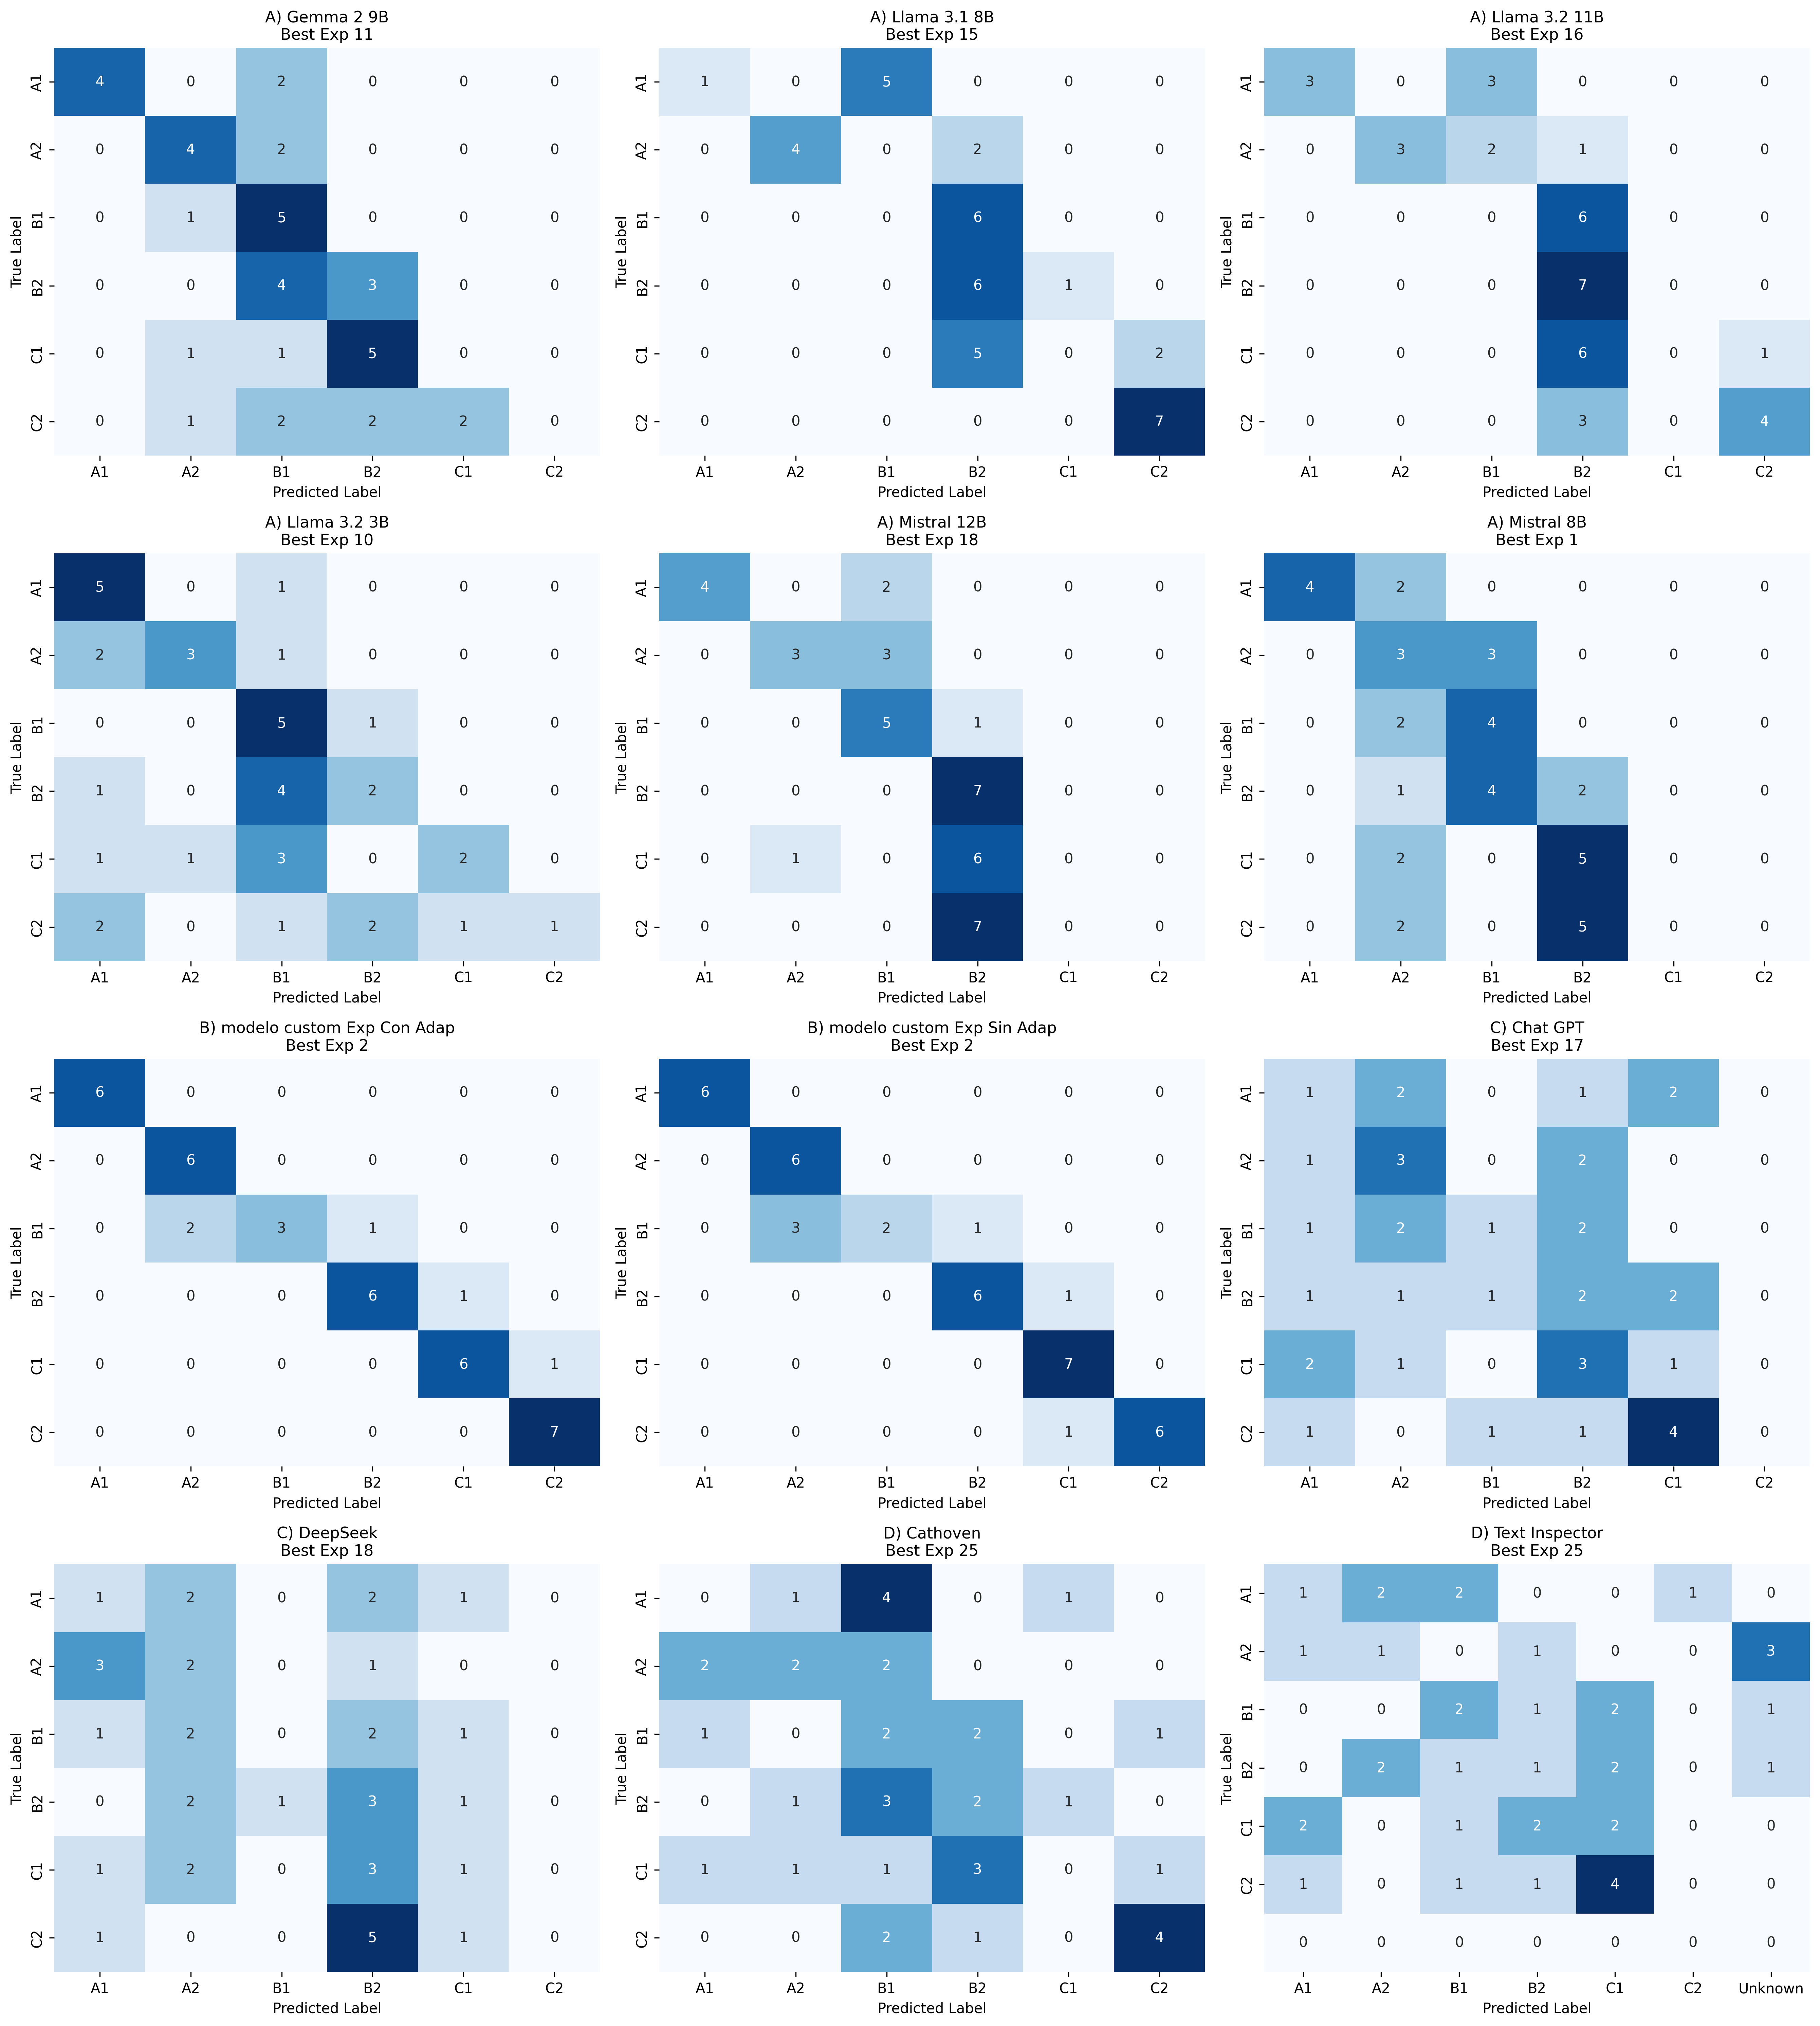
\includegraphics[width=\textwidth]{Graficos Tesis/custom_dataset_evaluacion_todas_matrices.png}
  \caption{Matriz de confucion de todos los modelos, con su mejor prompt segun Aproximated Acuraccy.}
  \label{fig:matriz_confucion}
\end{figure*}

\todo{Cambiar exp por prompt, cambiar titulo y orden de finetuning}


\subsubsection{Discusión}
\todo{agregar que tambien existe una "infra clasificacion" para el nivel C2, que un motivo puede ser al igual que A1 no hay suficiente material durante las estapas de pre-entrenamiento, y otra puede ser que a niveles mas altos se le atribuye textos mas largos y cuando existe un texto complejo, pero corto este es mal clasificado}

Nuestros experimentos muestran que los LLMs generativos (decoder-only) pueden identificar de manera confiable el nivel CEFR de un texto, especialmente cuando han sido fine-tuned. Los modelos ajustados superan sistemáticamente todas las estrategias basadas en prompting, incluso aquellas que incluyen descriptores del CEFR o listas de vocabulario por nivel. Si bien los ejemplos en contexto mejoran ligeramente el rendimiento en algunos modelos, tambien generan una desmejora en otros modelos, generando una variabilidad segun el modelo. De hecho, algunos modelos presentan tanta variabilidad en resultados que se vuelven poco confiables.

Tambien esta comparacion entre prompts muestra que si bien hay una variabilidad en los resultados mostrados por un modelo particular, este modelo tiene una tendencia a sobre-clasificar alguna clase, siendo la mayoria de los modelos probados el nivel B2.
Ademas las mejoras en rendimiento obtenidaspor los diferentes prompts nunca alcanzan las obtenidas mediante fine-tuning con cantidades relativamente pequeñas de datos etiquetados. Esto confirma la importancia de la adaptación específica a la tarea, incluso para modelos que requieren un amplio conocimiento lingüístico.

La cantidad y calidad de los datos etiquetados influyen fuertemente en el rendimiento. No obstante, los errores siguen siendo frecuentes en los niveles intermedios (especialmente B1 y B2). Nuestros modelos con fine-tuning, así como Cathoven y Text Inspector, presentan dificultades para identificar correctamente textos A1, que suelen ser clasificados erróneamente como A2 o B1. Esto probablemente refleja dos factores interrelacionados: la escasez de textos genuinamente simples en los corpus disponibles públicamente y la posibilidad de que los datos de pre entrenamiento contengan muchos menos ejemplos prototípicos de nivel A1 que de niveles intermedios o avanzados. A medida que aumenta la simplicidad, los modelos pueden depender en exceso de rasgos léxicos o estructurales que no son suficientemente distintivos cuando la dificultad absoluta es baja.

Otra observación importante es que el tamaño del modelo influye hasta cierto umbral: los modelos con menos de 8B parámetros se comportan de manera inconsistente y son más sensibles a la redacción del prompt, mientras que los modelos de 8B parámetros o más convergen hacia niveles de rendimiento similares.

Finalmente, nuestra comparación con herramientas listas para usar, como Text Inspector o Cathoven, y con LLMs propietarios como ChatGPT y DeepSeek, muestra que ninguno alcanza el rendimiento de los LLMs especializados y ajustados finamente. Estos resultados sugieren que los LLMs de código abierto y con pesos accesibles ofrecen una solución más robusta y controlable para canalizaciones de adaptación sensibles al nivel CEFR.

\subsubsection{Conclusiones}

Nuestro estudio muestra que los LLMs generativos de código abierto pueden identificar de manera confiable el nivel CEFR de los textos, siempre que sean ajustados de forma adecuada. Mientras que el zero-shot y el in-context prompting conducen a un rendimiento moderado y, en ocasiones, inestable, los modelos ajustados alcanzan niveles de exactitud mejores que algunos evaluadores CEFR de referencia, a pesar de haber sido entrenados con conjuntos de datos sustancialmente más pequeños. El tamaño del modelo resulta relevante solo hasta cierto umbral, ya que los modelos de 8B parámetros o más muestran perfiles de rendimiento similares. Asimismo, la disponibilidad de datos etiquetados diversos y bien curados, particularmente en los rangos bajos e intermedios del CEFR, desempeña un papel decisivo en la precisión global.

Las persistentes clasificaciones erróneas alrededor del nivel A1 y en el límite entre B1 y B2 reflejan tanto ambigüedades inherentes a la escala CEFR como la escasez de datos, y subrayan la necesidad continua de corpus más ricos y equilibrados.

\subsubsection{Trabajo Futuro}

El trabajo futuro se centrará principalmente en evaluar todos los modelos y herramientas sobre la partición de holdout. Además se desearía medir la variabilidad de los modelos en conjunto con los prompt, tomando sub muestras aleatorias del dataset.

Como objetivos a largo plazo sería ampliar los conjuntos de datos de entrenamiento, agregando más datasets que se encuentran disponibles en internet (edia), corrigiendo de forma manual o semi-automatica el dataset de kaggle. Analizar los resultados con los métodos y métricas de la shared task TSAR 2025, agregando la herramienta de clasificación de la competencia. Además de explorar estrategias de fine-tuning más expresivas, como el instruction tuning o los métodos de ajuste eficiente de parámetros, que permitan capturar mejor matices lingüísticos sutiles. 

Finalmente, incorporar corpus multilingües alineados con el CEFR y evaluar la capacidad de generalización cruzada entre lenguas podría ayudar a establecer modelos más robustos y agnósticos al idioma para el control de legibilidad y sistemas de aprendizaje de lenguas adaptativos.
